	\subsection{Output fluxes clustering}

		\subsubsection{K-Means}
			
			As K-Means allows for the number of clusters to be defined, and we know that there are 4 in the original dataset, K-Means is used to find 128 clusters.
			
			\begin{table}[h!]
				\centering
				\begin{tabular}{|c|c|c|}
					\hline
					& \textbf{Number of clusters} & \textbf{Number of initializations}\\
					\hline
					\textbf{Original Output fluxes} & 128 & 100\\
					\hline
				\end{tabular}
				\caption{K-Means hyperparameter configuration for output fluxes clustering}
			\end{table}
		
			The results are the following:
			
			\begin{figure*}[ht!]
				\centering
				\subfloat[Original cluster densities]{%
					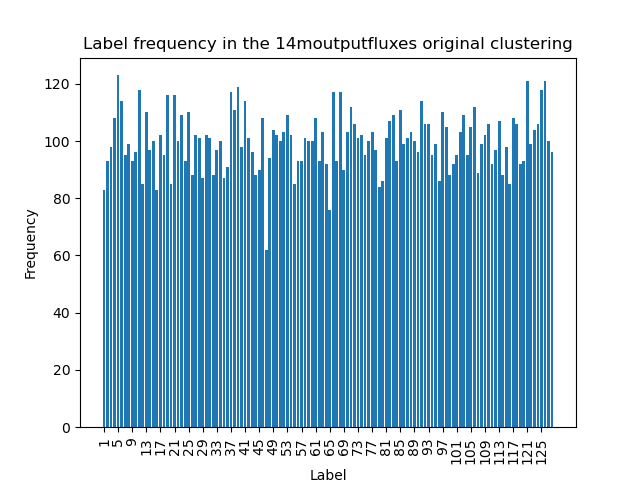
\includegraphics[width=0.45\textwidth]{mdid-14moutputfluxesoriginaldensity.png}}
				\hspace{\fill}
				\subfloat[K-Means clusters densities]{%
					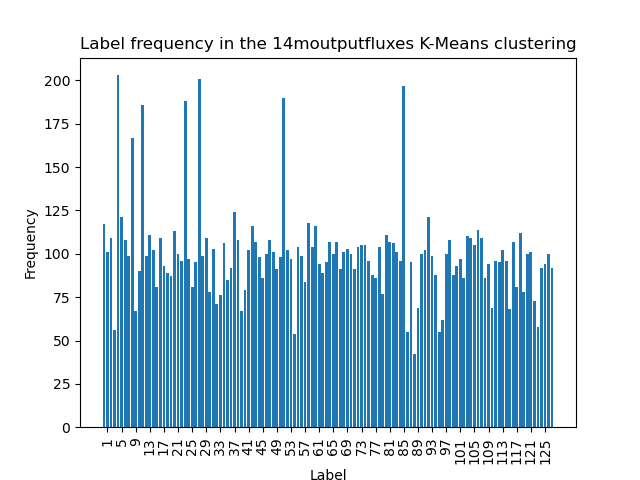
\includegraphics[width=0.45\textwidth]{mdid-14moutputfluxesK-Meansdensity.png}}\\
					
				\subfloat[Original cluster samples]{%
					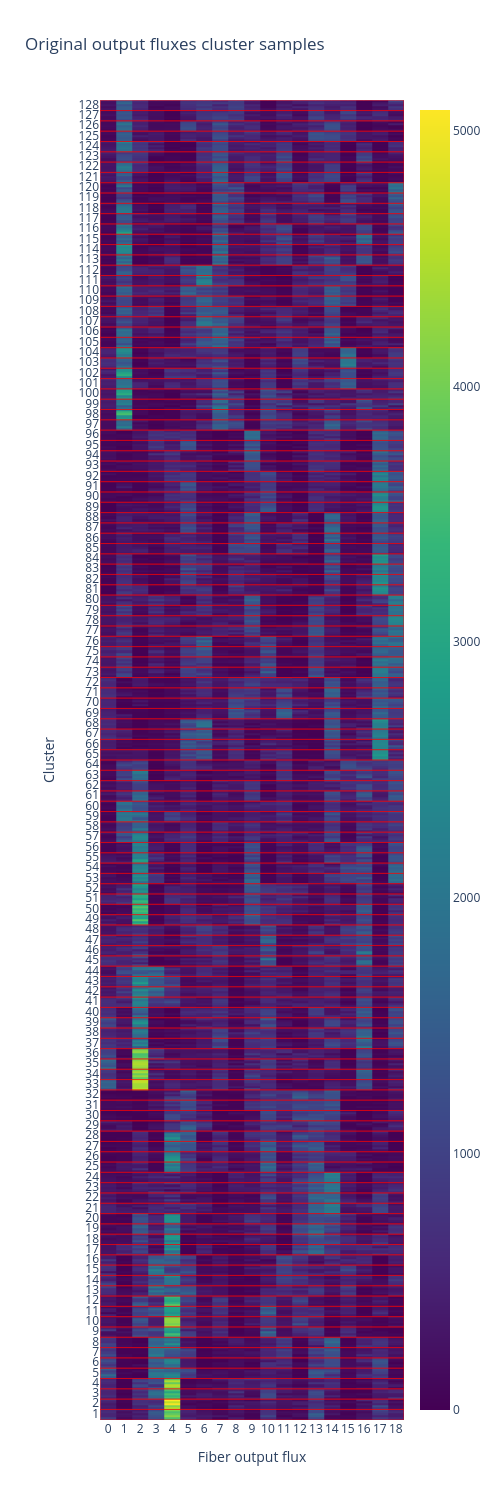
\includegraphics[width=0.4\textwidth]{mdid-14moutputfluxesoriginalgridclusters.png}}
				\hspace{\fill}
				\subfloat[K-Means cluster samples]{%
					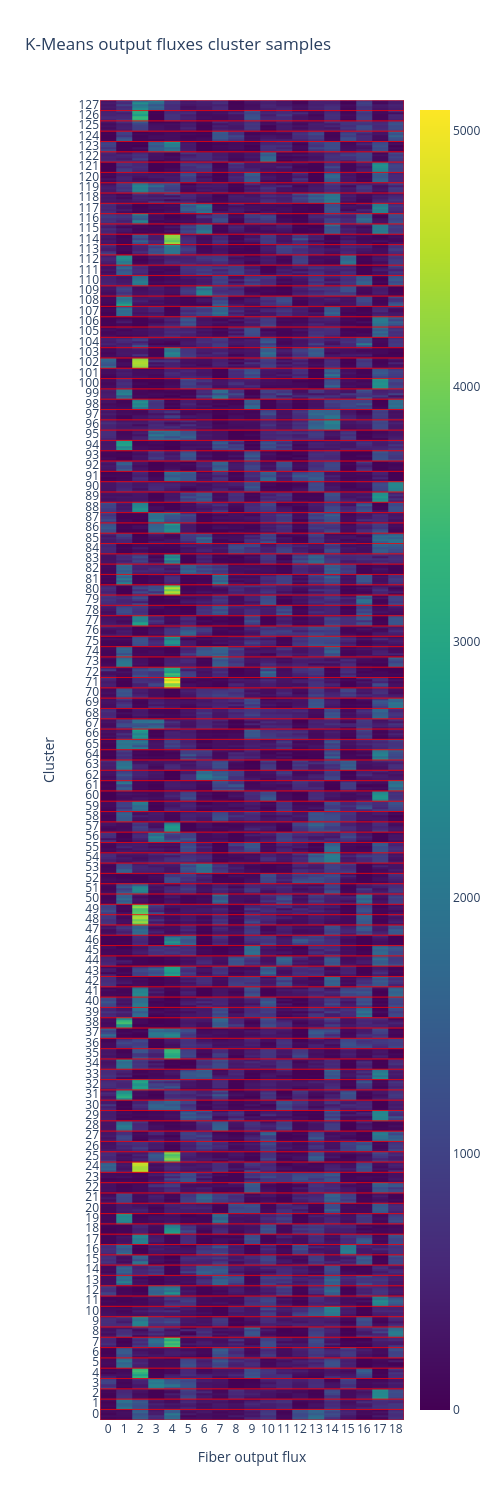
\includegraphics[width=0.4\textwidth]{mdid-14moutputfluxesK-Meansgridclusters.png}}
				\caption{Comparison between original clustering and K-Means clustering from original Output fluxes}
			\end{figure*}
			\FloatBarrier
		
		\subsubsection{DBSCAN}
			
			A configuration that outputs 4 clusters is searched
			
			\begin{table}[h!]
				\centering
				\begin{tabular}{|c|c|c|}
					\hline
					& \textbf{Number of neighbours} & \textbf{Epsilon}\\
					\hline
					Original Output fluxes & 3 & 412\\
					\hline
				\end{tabular}
				\caption{DBSCAN hyperparameter configuration for Output fluxes clustering}
			\end{table}
		
			The results are the following:
			
			\begin{figure*}[ht!]
				\centering
				\subfloat[Original cluster densities]{%
					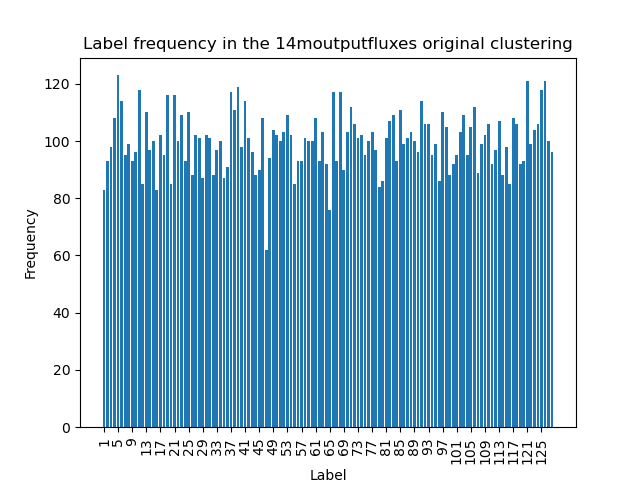
\includegraphics[width=0.45\textwidth]{mdid-14moutputfluxesoriginaldensity.png}}
				\hspace{\fill}
				\subfloat[DBSCAN clusters densities]{%
					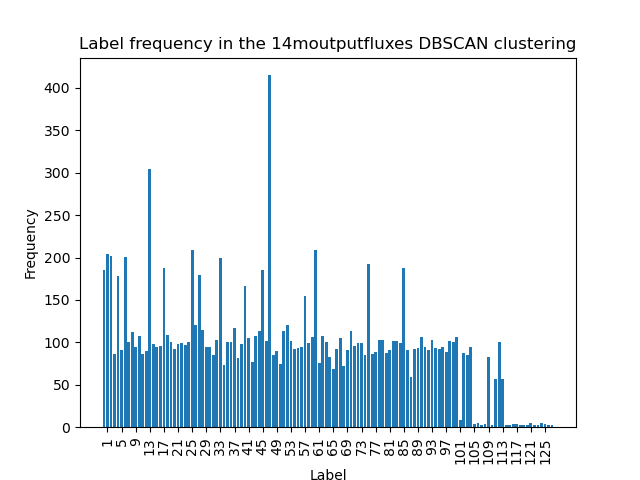
\includegraphics[width=0.45\textwidth]{mdid-14moutputfluxesDBSCANdensity.png}}\\
					
				\subfloat[Original cluster samples]{%
					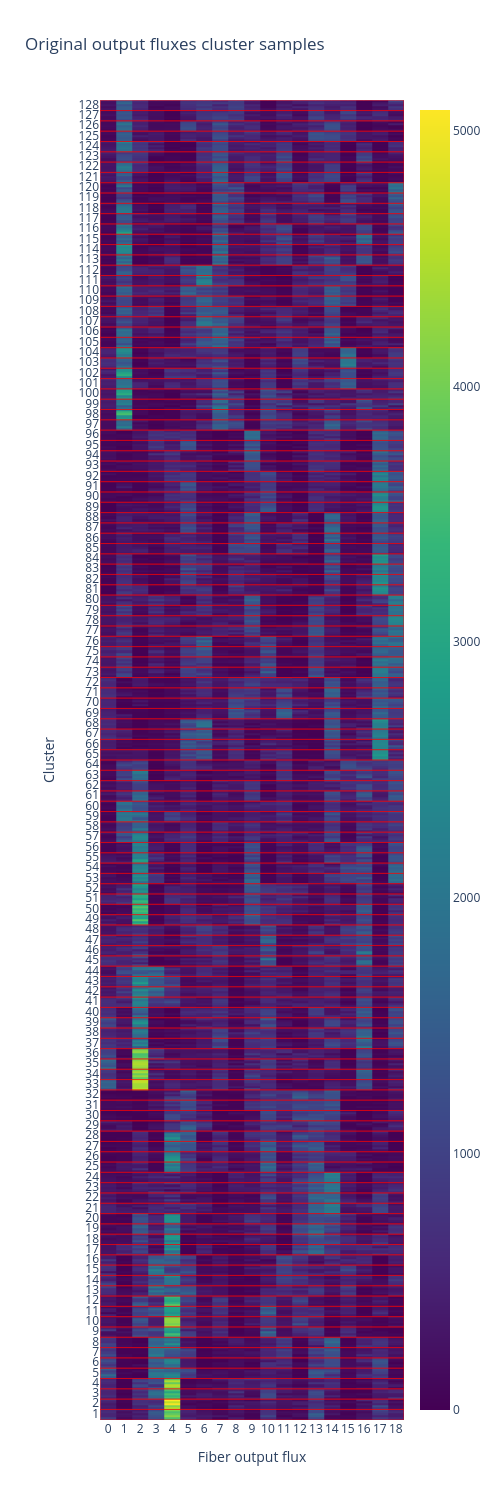
\includegraphics[width=0.4\textwidth]{mdid-14moutputfluxesoriginalgridclusters.png}}
				\hspace{\fill}
				\subfloat[DBSCAN cluster samples]{%
					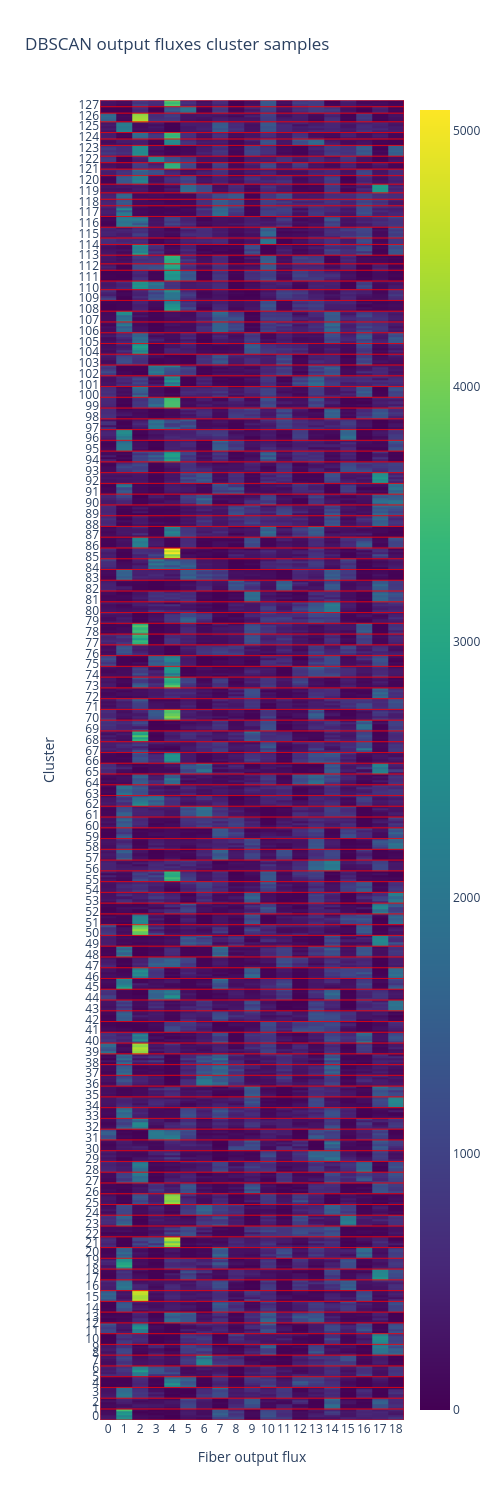
\includegraphics[width=0.4\textwidth]{mdid-14moutputfluxesDBSCANgridclusters.png}}
				\caption{Comparison between original clustering and DBSCAN clustering}
			\end{figure*}
			\FloatBarrier
		
		\subsubsection{HDBSCAN}
			
			A configuration that outputs 4 clusters is searched.
			
			\begin{table}[h!]
				\centering
				\begin{tabular}{|c|c|c|}
					\hline
					& \textbf{Minimum cluster size} \\
					\hline
					Original Output fluxes & 4 \\
					\hline
				\end{tabular}
				\caption{HDBSCAN hyperparameter configuration for Output fluxes clustering}
			\end{table}
			\FloatBarrier
			
			The results are the following:
			
			\begin{figure*}[ht!]
				\centering
				\subfloat[Original cluster densities]{%
					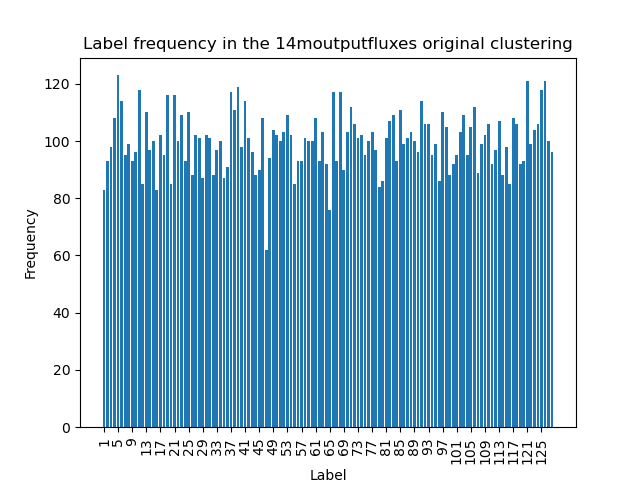
\includegraphics[width=0.45\textwidth]{mdid-14moutputfluxesoriginaldensity.png}}
				\hspace{\fill}
				\subfloat[HDBSCAN clusters densities]{%
					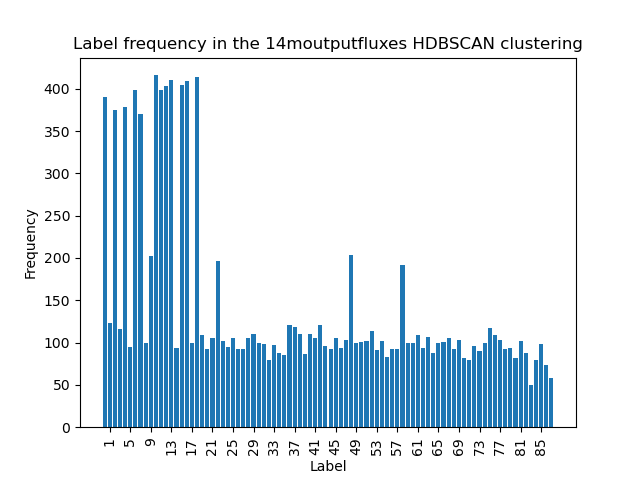
\includegraphics[width=0.45\textwidth]{mdid-14moutputfluxesHDBSCANdensity.png}}\\
					
				\subfloat[Original cluster samples]{%
					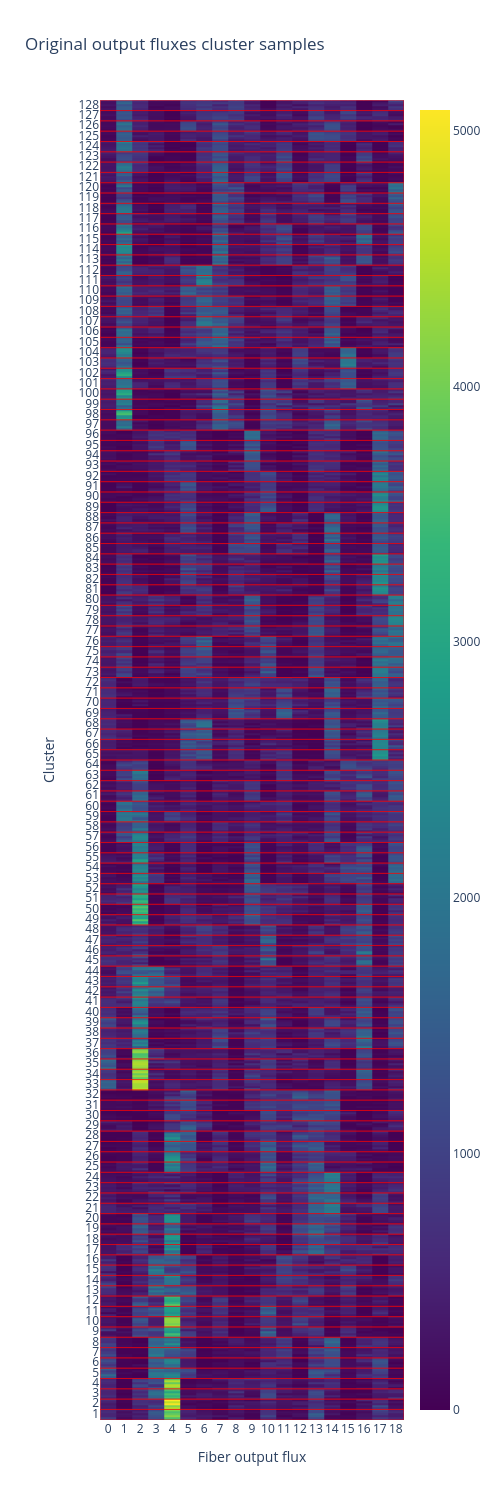
\includegraphics[width=0.4\textwidth]{mdid-14moutputfluxesoriginalgridclusters.png}}
				\hspace{\fill}
				\subfloat[HDBSCAN cluster samples]{%
					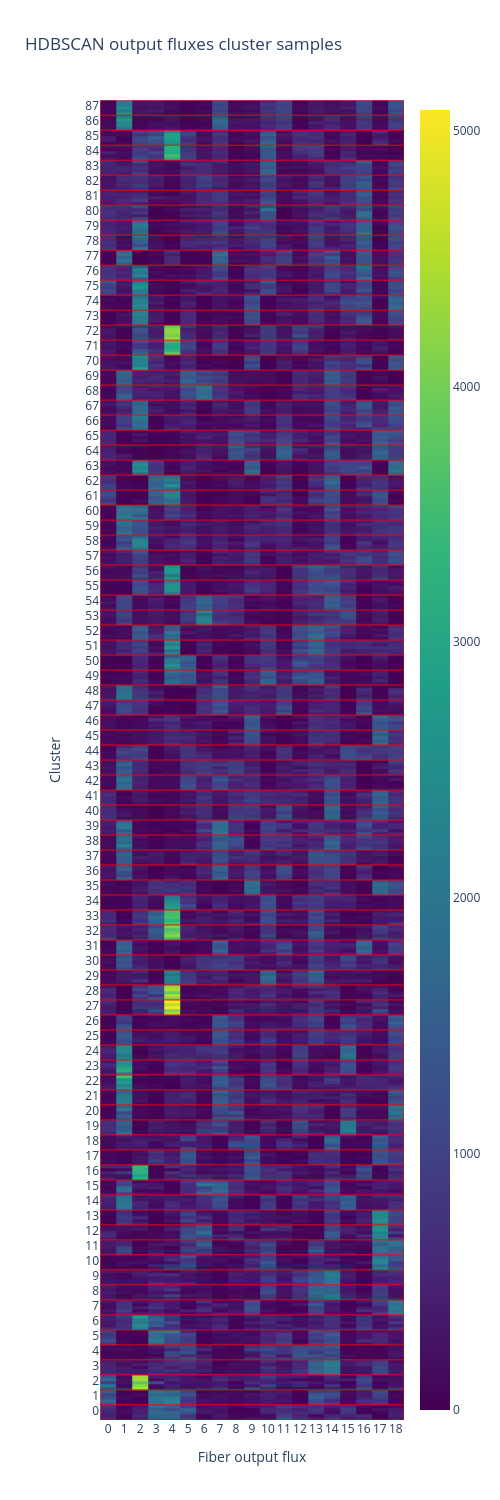
\includegraphics[width=0.4\textwidth]{mdid-14moutputfluxesHDBSCANgridclusters.png}}
				\caption{Comparison between original clustering and HDBSCAN clustering}
			\end{figure*}
			\FloatBarrier
		
		\subsubsection{Agglomerative clustering}
			\begin{table}[h!]
				\centering
				\begin{tabular}{|c|c|}
					\hline
					 & \textbf{Number of clusters} \\
					\hline
					Original Output fluxes & 128 \\
					\hline
				\end{tabular}
				\caption{Agglomerative hyperparameter configuration for Output fluxes clustering}
			\end{table}
			\FloatBarrier
			The results are the following:
			
			\begin{figure*}[ht!]
				\centering
				\subfloat[Original cluster densities]{%
					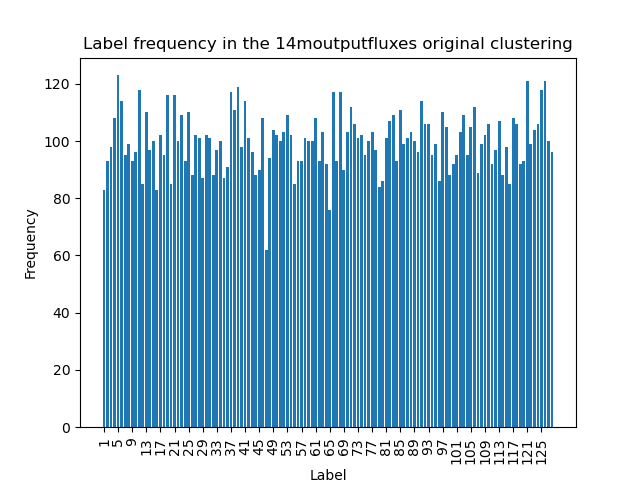
\includegraphics[width=0.45\textwidth]{mdid-14moutputfluxesoriginaldensity.png}}
				\hspace{\fill}
				\subfloat[Agglomerative clusters densities]{%
					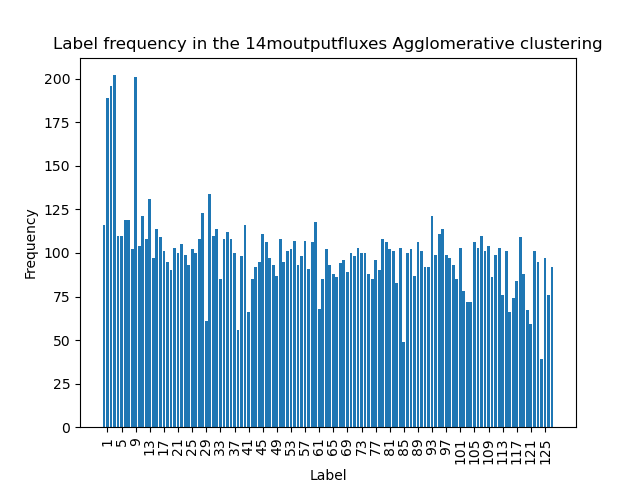
\includegraphics[width=0.45\textwidth]{mdid-14moutputfluxesAgglomerativedensity.png}}\\
					
				\subfloat[Original cluster samples]{%
					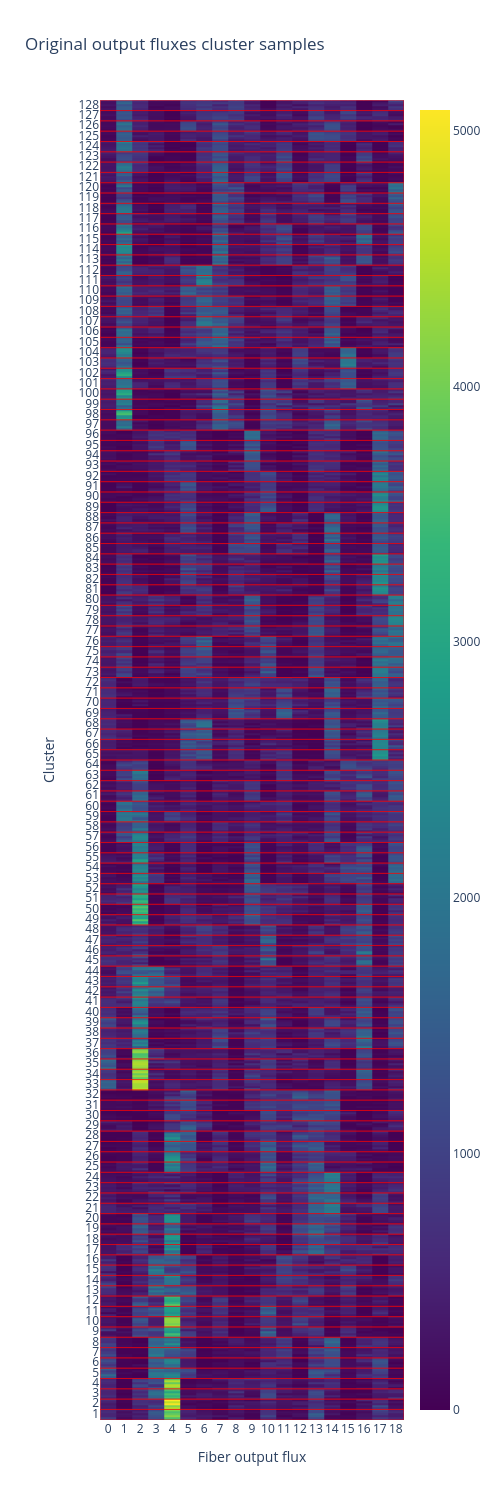
\includegraphics[width=0.4\textwidth]{mdid-14moutputfluxesoriginalgridclusters.png}}
				\hspace{\fill}
				\subfloat[Agglomerative cluster samples]{%
					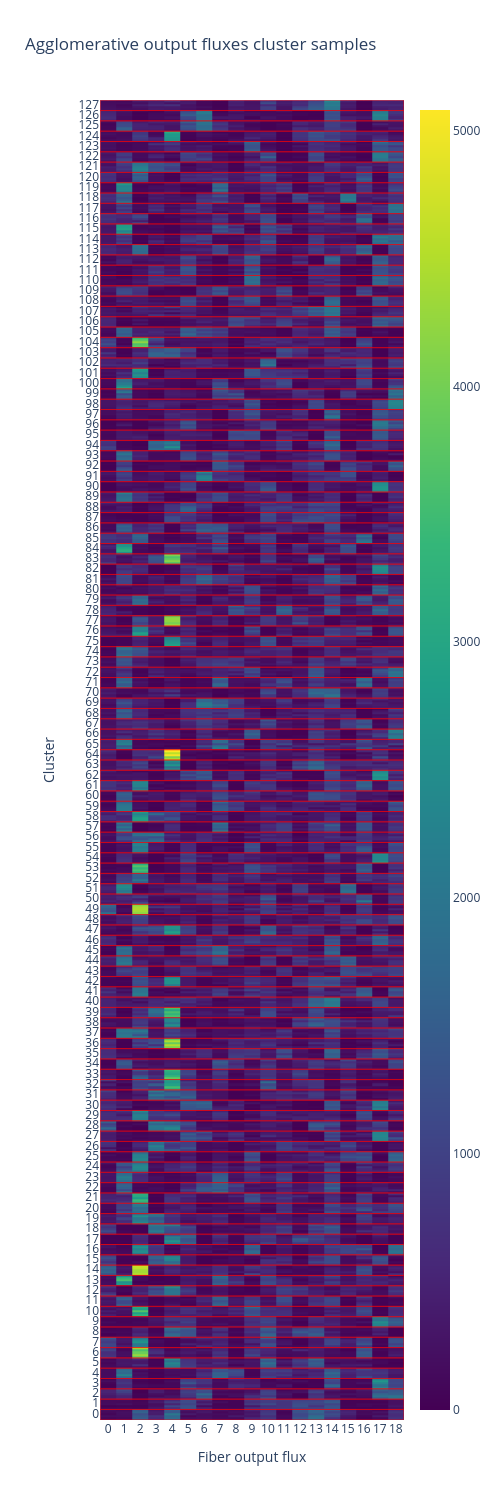
\includegraphics[width=0.4\textwidth]{mdid-14moutputfluxesAgglomerativegridclusters.png}}
				\caption{Comparison between original clustering and Agglomerative clustering}
			\end{figure*}
			\FloatBarrier
		
		\subsubsection{Summary}
			\begin{figure*}[ht!]
				\centering
				\subfloat[Original cluster densities]{%
					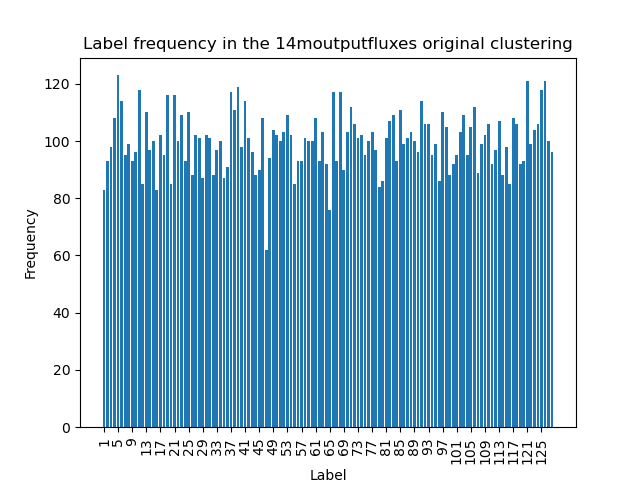
\includegraphics[width=0.18\textwidth]{mdid-14moutputfluxesoriginaldensity.png}}
				\hspace{\fill}
				\subfloat[K-means cluster densities]{%
					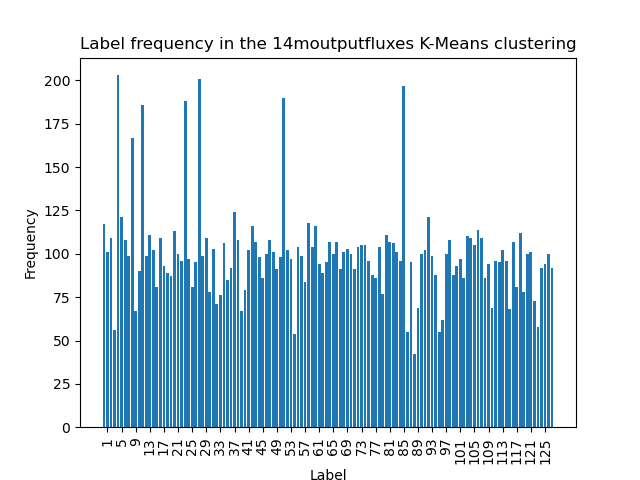
\includegraphics[width=0.18\textwidth]{mdid-14moutputfluxesK-Meansdensity.png}}
				\hspace{\fill}
				\subfloat[DBSCAN cluster densities]{%
					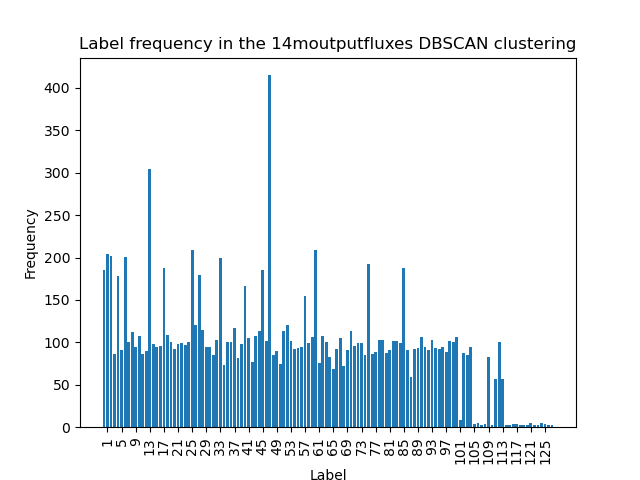
\includegraphics[width=0.18\textwidth]{mdid-14moutputfluxesDBSCANdensity.png}}
				\hspace{\fill}
				\subfloat[HDBSCAN cluster densities]{%
					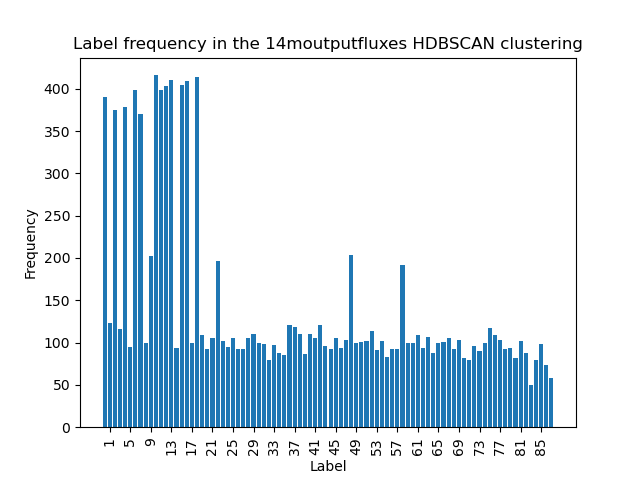
\includegraphics[width=0.18\textwidth]{mdid-14moutputfluxesHDBSCANdensity.png}}
				\hspace{\fill}
				\subfloat[Agglomerative cluster densities]{%
					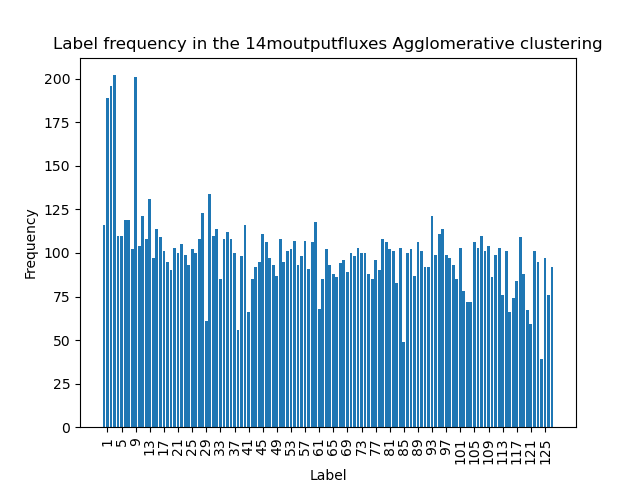
\includegraphics[width=0.18\textwidth]{mdid-14moutputfluxesAgglomerativedensity.png}}
				\\
				
				\subfloat[Original cluster samples]{%
					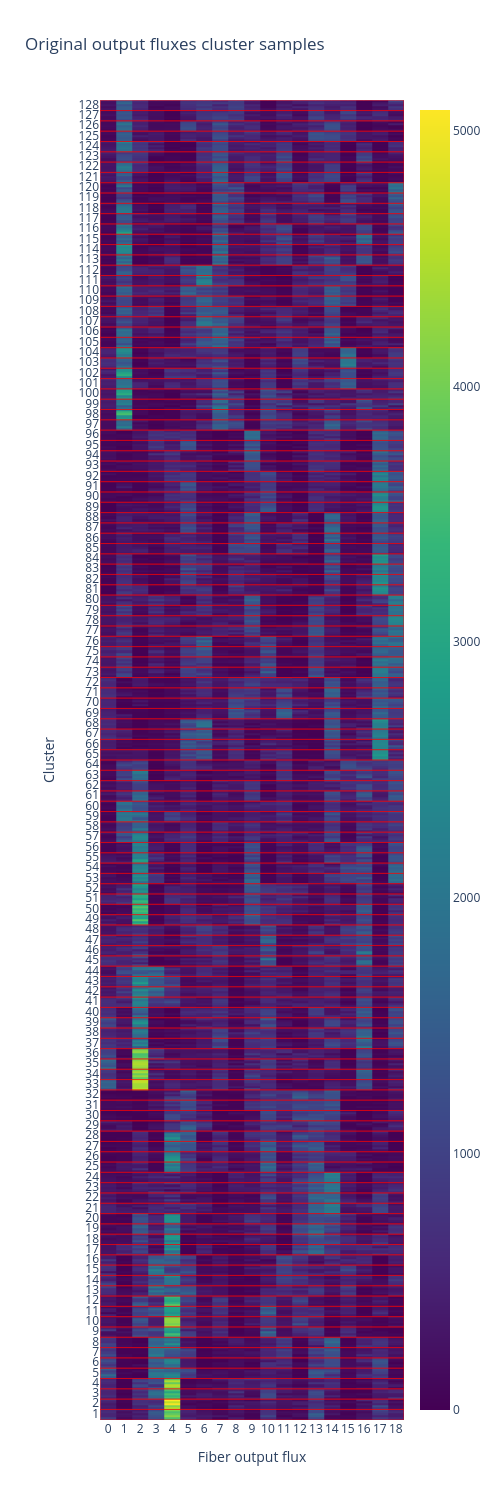
\includegraphics[width=0.18\textwidth]{mdid-14moutputfluxesoriginalgridclusters.png}}
				\hspace{\fill}
				\subfloat[K-means cluster samples]{%
					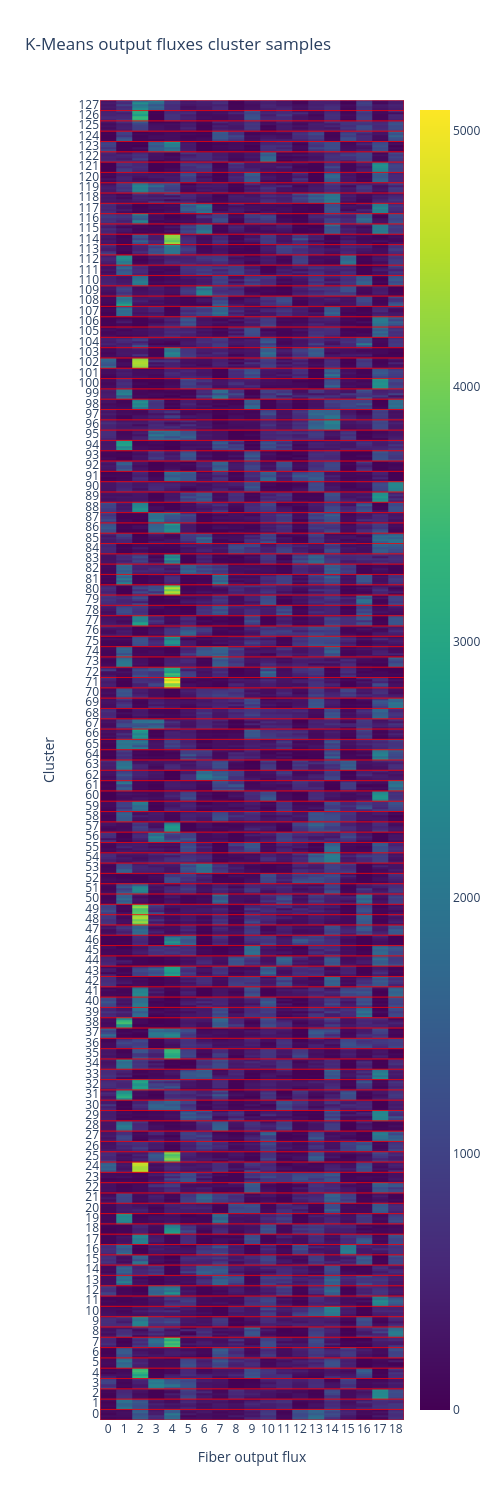
\includegraphics[width=0.18\textwidth]{mdid-14moutputfluxesK-Meansgridclusters.png}}
				\hspace{\fill}
				\subfloat[DBSCAN cluster samples]{%
					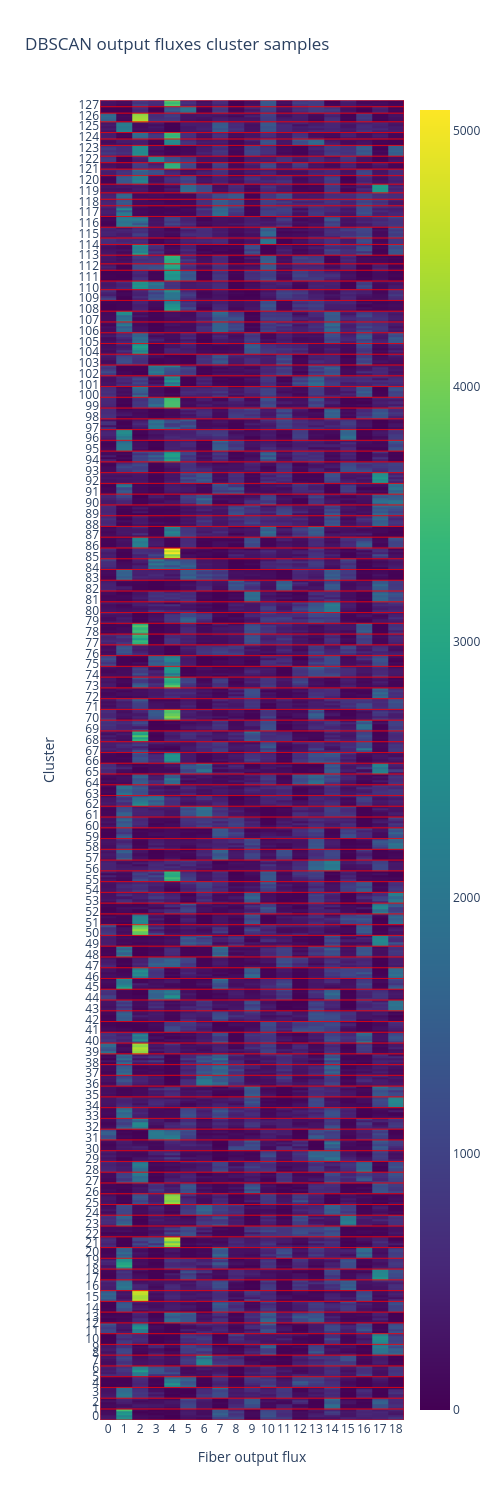
\includegraphics[width=0.18\textwidth]{mdid-14moutputfluxesDBSCANgridclusters.png}}
				\hspace{\fill}
				\subfloat[HDBSCAN cluster samples]{%
					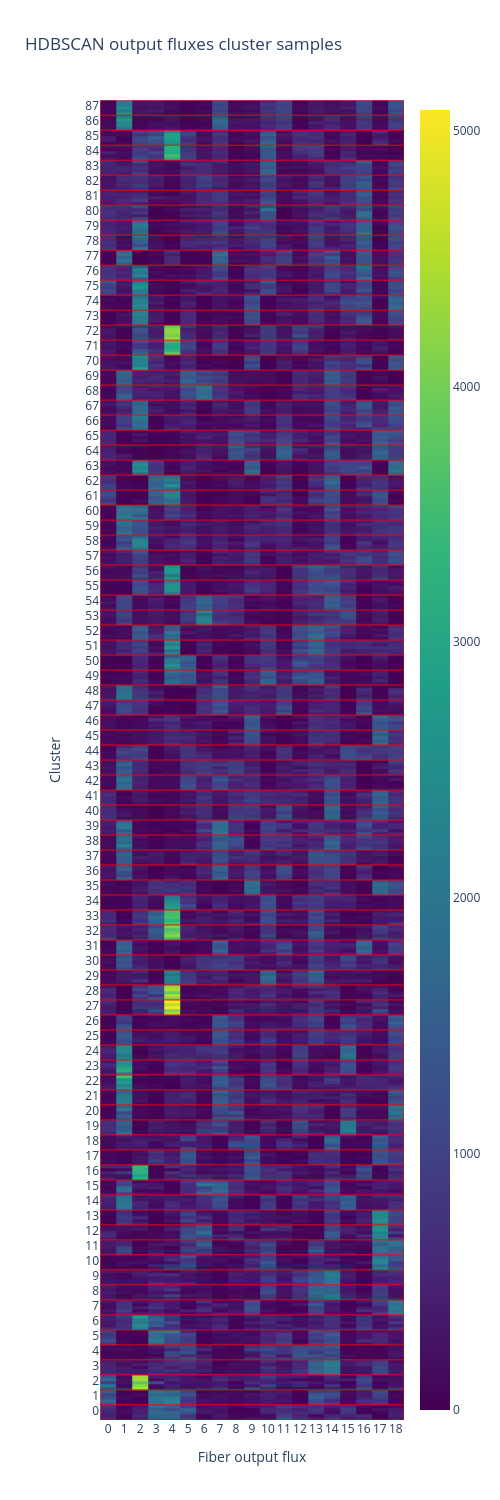
\includegraphics[width=0.18\textwidth]{mdid-14moutputfluxesHDBSCANgridclusters.png}}
				\hspace{\fill}
				\subfloat[Agglomerative cluster samples]{%
					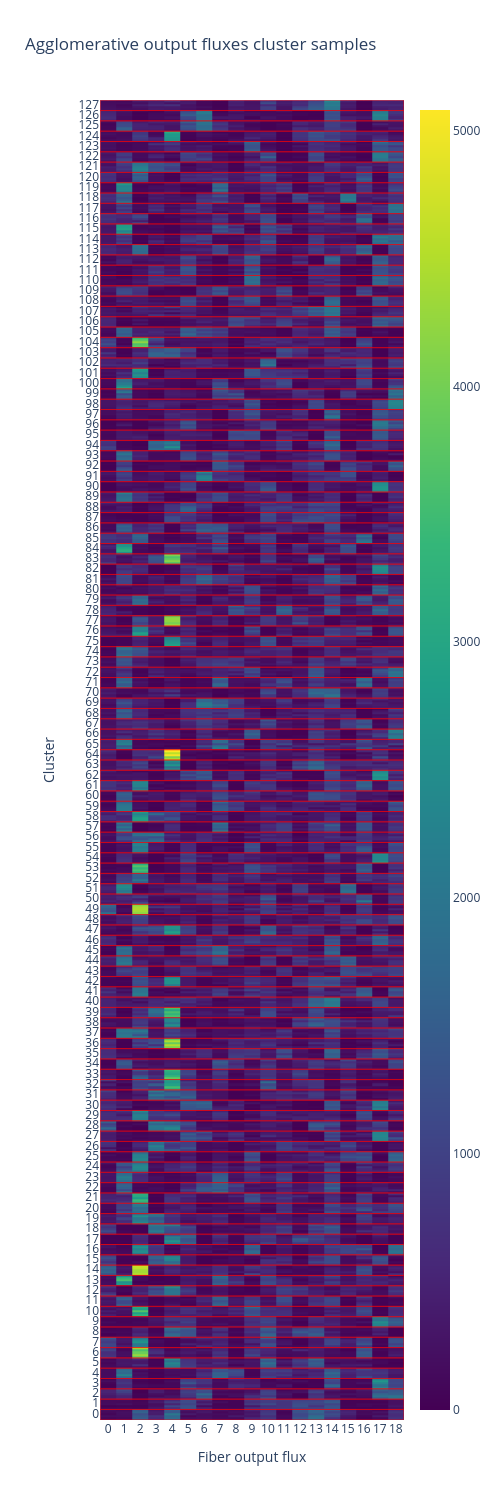
\includegraphics[width=0.18\textwidth]{mdid-14moutputfluxesAgglomerativegridclusters.png}}
				
				\caption{Comparison between clustering Output fluxes algorithms}
			\end{figure*}
		\FloatBarrier
		
		\begin{table}[h!]
    			\centering
    			\begin{tabular}{|c|c|c|c|c|c|}
        			\hline
        			& \textbf{Original} & \textbf{K-Means} & \textbf{DBSCAN} & \textbf{HDBSCAN} & \textbf{Agglomerative} \\
        			\hline
        			\textbf{Original} & \diagbox{}{} & 0.969 & 0.939 & 0.925 & 0.982 \\
       			\hline
        			\textbf{K-Means} &  & \diagbox{}{} & 0.929 & 0.923 & 0.970\\
        			\hline
        			\textbf{DBSCAN} &  &  & \diagbox{}{} & 0.922 & 0.938\\
        			\hline
        			\textbf{HDBSCAN} &  &  &  & \diagbox{}{} & 0.925\\
       			\hline
    			\end{tabular}
    			\caption{Normalized Mutual Information between original Output fluxes clusters}
		\end{table}